\section{Résultats}

Comme mentionné en introduction, nous avons testé trois méthodes de vectorisation : TF-IDF, doc2vec et BERT
Nous avons utilisé ces vecteurs pour entraîner et comparer 4 modèles différents : Régression logistique, SVM, Random Forest et Perceptron.

\subsection{Vecteurs BERT}

\begin{figure}[t]
  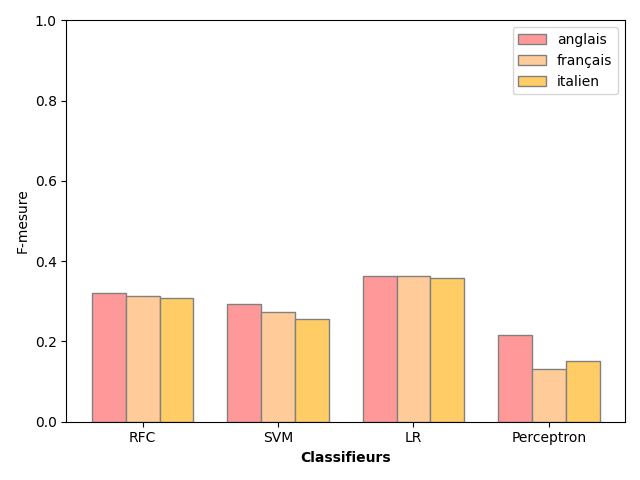
\includegraphics[width=\columnwidth]{assets/comparaison_metriques_bert.png}
  \caption{Résultats obtenus avec les vecteurs BERT.}
  \label{fig:bert_comparison}
\end{figure}

La figure~\ref{fig:bert_comparison} montre qu'avec les vecteurs BERT, la régression logistique obtient les meilleurs résultats dans les trois langues.

\subsection{Vecteurs doc2vec}

\begin{figure}[t]
  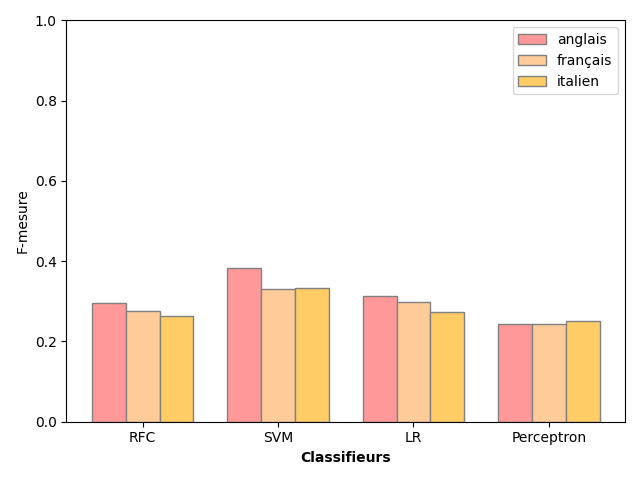
\includegraphics[width=\columnwidth]{assets/comparaison_metriques_doc2vec.png}
  \caption{Résultats obtenus avec les vecteurs doc2vec.}
  \label{fig:doc2vec_comparison}
\end{figure}

Comme on peut le voir sur la figure~\ref{fig:doc2vec_comparison}, avec les vecteurs doc2vec, c'est le SVM qui obtient les meilleurs résultats dans les trois langues.

\subsection{Vecteurs TF-IDF}

\begin{figure}[t]
  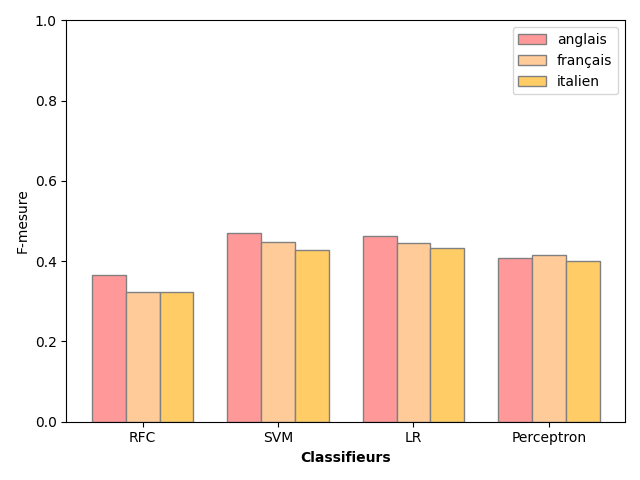
\includegraphics[width=\columnwidth]{assets/comparaison_metriques_tfidf.png}
  \caption{Résultats obtenus avec les vecteurs TF-IDF.}
  \label{fig:tfidf_comparison}
\end{figure}

Les meilleurs résultats que nous ayons obtenus sont ceux avec un vectorisation tf-idf.
On peut voir sur la figure~\ref{fig:tfidf_comparison} que nous avons obtenu au mieux : 0.46 en anglais avec un SVM, 0.43 en italien avec une régression linéaire et 0.44 en français avec un SVM.